
To precisely define what behavior the \openshmem interface guarantees for both users and implementers, this section formally defines an API-level memory model. An API-level model builds upon a programming language-level (PL-level) memory model, and it defines how API operations impact memory. This is useful for determining the ordering and visibility requirements for \openshmem memory accesses when implemented on any device, but it is of particular importance for devices like GPUs that have software managed caches requiring expensive bulk flush or invalidate actions to enforce memory ordering guarantees. Without a precisely specified memory model, API implementers and users may disagree on what behavior is guaranteed by the API, and this can lead to poor performance (too many bulk cache actions) or buggy code (too few bulk cache actions).

This section describes how \openshmem extends the C11 memory consistency model. C11 is chosen as an example because of its generality and ubiquity in the CPU domain, and because it forms the basis for common GPU programming languages (for example, CUDA, HIP). Section~\ref{subsubsec:api_pl_baseline} summarizes the baseline C11 memory model, Sections~\ref{subsubsec:api_model_overview}-\ref{subsubsec:api_integrate} describe how this programming language-level model is extended to provide API-level semantics for \openshmem, and Section~\ref{subsubsec:api_scoped} describes how the guarantees of the API-level model can be adapted for GPU memory models.

\subsubsection{Baseline PL-level Axiomatic Memory Model (C11)}\label{subsubsec:api_pl_baseline}

A memory consistency model (MCM) defines what values loads are allowed to return in a multi-threaded program. One common way to formally specify a MCM is via axioms over relations between events in a dynamic execution. Axiomatic formalization begins by considering all possible “candidate” executions of a parallel program. Loads may return the value of a conflicting store anywhere else in the execution, or the initial value at that memory location (i.e., allowing all possible reorderings). The model then defines relations between accesses in the candidate executions, and using axioms over these relations, defines which executions are legal (hence restricting which reorderings are allowed by the compiler or hardware).

The C11 memory model is defined axiomatically in the C11 specification \S5.1.2.4. Although many prior works aim to mathematize or improve this formalism, the intent here is simply to provide sufficient understanding to build upon it with the \openshmem API model.

Under the PL-level C11 memory model, events consist of reads (\EVENT{R}), writes (\EVENT{W}), atomic read-modify-writes (\EVENT{RMW}, which perform both a read and write to memory), and fences (\EVENT{F}). Events that access memory may be atomic or non-atomic. Atomic events are associated with a memory order which can be acquire, release, acquire-release, or relaxed. These memory orders determine how atomic accesses can legally synchronize (release and acquire are used with the source and destination of a synchronizing access pair, respectively). The following relations are defined over the events in a candidate execution, and will be used to derive API-level relations in Section~\ref{subsubsec:api_relations}:

\begin{itemize}
    \item \textbf{Sequenced before (\REL{sb}):} Relates memory events from the same thread based on the order they are evaluated (also called program order in some contexts)
    \item \textbf{Modification order (\REL{mo}):} A total ordering between all modifying accesses (writes or read-modify-writes) to the same memory location.
    \item \textbf{Reads-from (\REL{rf}):} Relates a write \EVENT{W} and any read \EVENT{R} to the same memory location such that \EVENT{R} returns the value written by \EVENT{W}.
    \item \textbf{Synchronizes-with (\REL{sw}):} Same as \REL{rf}, but also requires that \EVENT{W} and \EVENT{R} are atomic, \EVENT{W} has release or acquire-release memory order, and \EVENT{R} has acquire or acquire-release memory order (this relation is also called synchronization order in some contexts).
    \item \textbf{Happens-before (\REL{hb}):} Transitive closure of \relSW{} and \relSB{}.
\end{itemize}

Furthermore, a \textbf{data race} is defined as a relation between two accesses $A$ and $B$ where all of the following are true:
\begin{itemize}
    \item $A$ and $B$ access the same memory location.
    \item At least one access is a modifying access (write or read-modify-write).
    \item At least one access is not atomic.
    \item $A$ and $B$ are not related by \relHB{}.
\end{itemize}

Although the axiomatic model places no requirements on when each event must update or access physical memory, it prohibits executions that don't adhere to a set of constraints, and by extension it disallows any architecture or compilation scheme that can result in such an execution. Specifically, C11 constrains candidate execution with the following axioms:

\begin{itemize}
    \item $acyclic(hb)$: \relHB{} cannot have any cycles.
    \item $irreflexive(rf;hb)$: \relHB{} must be consistent with the \relRF{} relation.
    \item $irreflexive((rf^{-1})^{?};mo;rf^?;hb)$: \relHB{} must be consistent with \relMO{} between writes, as well as any reads that read from writes in \relMO{} (often called coherence requirement).
    \item $irreflexive(rf \cup (mo;mo;rf^{-1}) \cup (mo;rf))$: The read of an atomic read-modify-write access must always read the last value (in \relMO{}) written before the write of the read-modify-write access (often called RMW atomicity).
\end{itemize}

Finally, the C11 specification states that, if a data race exists in a candidate execution that satisfies the above axioms, then the program's behavior is undefined. If a data race does not exist, then the program's behavior must conform to one of the conforming candidate executions.

\begin{description}
\apinotes{Consume and sequential consistent memory orders are omitted from the above formalism for simplicity, but this does not impact how the PL-level semantics are extended for the API-level model.
Also, instead of the verbose prose axioms defined in the C11 specification, the C11 axioms are expressed above using the more concise (and equivalent) representation outlined by Batty et al. in "Overhauling SC atomics in C11 and OpenCL" (Symposium on the Principles of Programming Languages, 2016).}
\end{description}


\subsubsection{API-Level Memory Model Overview}\label{subsubsec:api_model_overview}

The \openshmem API-level memory model extends PL-level memory models like C11 to define how \openshmem operations interact with memory. PL-level models use acquire and release semantics to establish ordering relations between fine-grain loads, stores, and fences. The API-level memory model must additionally operate on coarse-grain API operations like \GET{}, \PUT{}, barrier, etc. that can execute asynchronously and involve multiple \acp{PE}.
Rather than defining allowed behavior by leveraging PL-level events and relations, we can more flexibly capture the higher level ordering requirements of \openshmem by defining new events and ordering relations. These can then be lowered to PL-level relations transparently to the programmer, enabling a wide range of backend implementations. We formalize allowed behavior by extending the axiomatic PL-level memory model to incorporate these new events and relations.

To describe the desired \openshmem behavior, the API-level memory model makes the following additions to the existing PL-level model:

\begin{enumerate}
	\item\label{mcmsteps:one} \textbf{\acp{PE} and operation events}: Section~\ref{subsubsec:api_pes_operations} introduces a new event type that corresponds to an API operation and a new memory location property that specifies the target \ac{PE}. This provides a basis for operation-level semantics across multiple \ac{PE} memories.
	\item\label{mcmsteps:two} \textbf{Per-operation observable accesses}: For each operation type, Section~\ref{subsubsec:api_observable} defines a set of observable memory accesses (these are not related to the initiating thread by \relSB{}). This enables asynchrony since a thread can continue execution while observable accesses execute in the background.
	\item\label{mcmsteps:four} \textbf{Fused collectives}: Section~\ref{subsubsec:api_fused} fuses matched collective operation calls into a single event. This supports multi-PE collective operations and establishes ordering across \acp{PE} even when there are no observable accesses.
	\item\label{mcmsteps:three} \textbf{API-level relations}: Section~\ref{subsubsec:api_relations} defines new API-level ordering relations over operation events and their observable accesses that will constrain \openshmem memory ordering. This allows the programmer to explicitly enforce ordering of asynchronous operations using the ordering and synchronization operations provided by \openshmem. These relations are illustrated in Section~\ref{subsubsec:api_relations_example}.
	\item\label{mcmsteps:five} \textbf{Updated relations, axioms}: Section~\ref{subsubsec:api_integrate} updates the PL-level memory model axioms to incorporate these new events and relations. By extending existing relations and axioms (e.g., \relHB{}, data races) for the API level, we establish a memory model that formalizes \openshmem ordering requirements.
\end{enumerate}

After defining how \openshmem extends the C11 memory model, Section~\ref{subsubsec:api_scoped} describes how the addition of scoped synchronization in GPU memory models impacts the API-level model.

\subsubsection{PEs and Operation Events}\label{subsubsec:api_pes_operations}

When defining behavior at the \openshmem API level, there are two key differences in program representation relative to a PL-level program. First, \openshmem applications span multiple \acp{PE}, each of which has its own local memory space. Therefore, the PL-level definition of memory location is extended to include both the \ac{PE}-local memory address and the \ac{PE} ID. Normal memory accesses can access memory locations on the local \ac{PE}, or on a remote \ac{PE} if \FUNC{shmem\_ptr} is used. \openshmem operations may trigger accesses to the local \ac{PE}’s memory and/or the memory of remote \acp{PE}. Dynamic memory accesses in an execution are only considered to access the same memory location if both the local memory address and \ac{PE} ID attributes match (impacting the definitions of of \relMO{} and \relRF{}).

Second, since the \openshmem API does not define the underlying PL-level implementation, API operations do not resolve to a function consisting of PL-level events. Thus, these operations must be treated as a new type of primitive in the API-level memory model: the operation event. An operation event specifies its type, and each type defines the set of minimum observable accesses triggered by the operation (described next). Operation events participate in \relSB{} and derived relations, similar to normal thread access events. Although operation events may be associated with separate memory access events (see Section~\ref{subsubsec:api_observable}), the operation events themselves do not participate directly in access-based relations like \relMO{}, \relRF{}, and \relSW{}.

\subsubsection{Per-Operation Observable Accesses}\label{subsubsec:api_observable}

For the purposes of the API memory model, each \openshmem operation type defines the minimum set of observable memory accesses performed by the operation. These accesses are considered to be ``issued'' by the associated operation. These accesses must occur as part of the operation, however the API-level model places no constraints on the thread that executes observable accesses (i.e., they may or may not be executed by the initiating thread), and it does not prevent an implementation from performing other accesses (e.g., for implementation-internal synchronization, buffering, etc. -- although data accessed in this way should never be accessed by code external to the implementation).
Observable accesses have the same semantics as normal accesses and take part in the same relations, with two exceptions: 
\begin{enumerate}
  \item There is no \relSB{} relationship between observable accesses issued by an API operation and any other event in the thread that initiated the operation. Instead, Section~\ref{subsubsec:api_relations} defines the relations that constrain ordering at the API level. Note, however, that the operation event that issues these observable accesses \textit{does} form a \relSB{} relationship with other events issued by the initiating thread.
  \item There are no synchronization semantics (atomic, acquire/release ordering) associated with observable accesses. Although the accesses may be lowered to PL-level accesses with these semantics, at the API level, ordering relations and data race conditions are defined a the level of the operation that issues them (see Sections~\ref{subsubsec:api_relations} and~\ref{subsubsec:api_integrate}, respectively).
\end{enumerate}
%In addition, accesses performed by an implementation that are not included in the observable set must not modify data that may be observed from application code external to \openshmem operation implementations. 

Table~\ref{table:api_observable} defines the observable accesses performed for each \openshmem operation. Each access denotes the memory location as well as the \ac{PE} it targets ($my\_pe$ refers to the \ac{PE} of the initiating thread). 
In many cases, control and compute pseudocode are included to define which memory locations are accessed, which values are stored, and which values must eventually be loaded (pseudocode rather than C11 is used here because it allows clearer specification of where memory accesses are required).
However, this single-threaded control flow does not constrain the actual implementation and does not necessarily imply a total \relSB{} ordering between observable accesses. Within an operation, \relSB{} is defined to exist only between observable accesses when there is a true control or data dependency between two accesses (i.e., no \relSB{} relation across independent iterations of a loop). 
Specifically, $(A, B) \in sb$ only if $A$ and $B$ are observable accesses issued by the same operation and one of the following is true:
    \begin{itemize}
        \item $B$ takes a value derived from $A$ as an operand.
        \item $B$ has a control dependency on the result of $A$ such that $A$'s evaluation determines whether $B$ will occur.
	\item $B$ has an ordering dependency $A$. This type of dependency currently exists only in blocking and non-blocking \emph{put-with-signal} operations where the final store to $sig\_addr$ is ordered after all prior observable accesses to source and dest.
    \end{itemize} 
Many operations have no visible accesses (e.g., memory ordering routines, whose semantics are defined by the API-level relations described in Section~\ref{subsubsec:api_relations}). 
In addition, synchronization semantics for observable accesses in the API model are defined at a higher level than in the PL model. Rather than associating atomic semantics and acquire/release ordering for each observable accesses that may be involved in synchronization, we instead associate semantics at the level of the issuing operation (see API Synchronizes-With in \ref{subsubsec:api_relations}).


\normalsize
\begin{longtable}{|m{0.27\textwidth}|m{0.68\textwidth}|}
\hline
\textbf{Operation Category} & \textbf{Operation Type, Params, and Observable Accesses}
\tabularnewline\hline
\endhead
%%
Remote Access Routine
    & \begin{BVerbatim}
shmem_put[_nbi](dest, source, nelems, pe):
  for i in nelems:
    R1 = LD source[i], my_pe
    ST R1 -> dest[i], pe
    \end{BVerbatim}
    \tabularnewline\hline
Remote Access Routine
    & \begin{BVerbatim}
shmem_p(dest, value, pe):
  ST value -> dest, pe
    \end{BVerbatim}
    \tabularnewline\hline
Remote Access Routine
    & \begin{BVerbatim}
shmem_iput(dest, source, dst, sst, nelems, pe):
  for i in nelems:
    R1 = LD source[i*sst], my_pe
    ST R1 -> dest[i*dst], pe
    \end{BVerbatim}
    \tabularnewline\hline
Remote Access Routine
    & \begin{BVerbatim}
shmem_get[_nbi](dest, source, nelems, pe):
  for i in nelems:
    R1 = LD source[i], pe
    ST R1 -> dest[i], my_pe
    \end{BVerbatim}
    \tabularnewline\hline
Remote Access Routine
    & \begin{BVerbatim}
shmem_g(source, pe):
  return LD source, pe
    \end{BVerbatim}
    \tabularnewline\hline
Remote Access Routine
    & \begin{BVerbatim}
shmem_iget(dest, source, dst, sst, nelems, pe):
  for i in nelems:
    R1 = LD source[i*sst], pe
    ST R1 -> dest[i*dst], my_pe
    \end{BVerbatim}
    \tabularnewline\hline
Atomic Memory Operation
    & \begin{BVerbatim}
shmem_atomic_fetch(source, pe):
  return LD source, pe
    \end{BVerbatim}
    \tabularnewline\hline
Atomic Memory Operation
    & \begin{BVerbatim}
shmem_atomic_set(dest, value, pe):
  ST value -> dest, pe
    \end{BVerbatim}
    \tabularnewline\hline
Atomic Memory Operation
    & \begin{BVerbatim}
shmem_atomic_compare_swap(dest, cond, value, pe):
  R1 = LD dest, pe
  if R1 == cond:
    ST value -> dest, pe
  return R1
    \end{BVerbatim}
    \tabularnewline\hline
Atomic Memory Operation
    & \begin{BVerbatim}
shmem_atomic_swap(dest, value, pe):
  R1 = LD dest, pe
  ST value -> dest, pe
  return R1
    \end{BVerbatim}
    \tabularnewline\hline
Atomic Memory Operation
    & \begin{BVerbatim}
shmem_atomic_fetch_inc(dest, pe):
  R1 = LD dest, pe
  R2 = R1 + 1
  ST R2 -> dest, pe
  return R1
    \end{BVerbatim}
    \tabularnewline\hline
Atomic Memory Operation
    & \begin{BVerbatim}
shmem_atomic_inc(dest, pe):
  R1 = LD dest, pe
  R2 = R1 + 1
  ST R2 -> dest, pe
    \end{BVerbatim}
    \tabularnewline\hline
Atomic Memory Operation
    & \begin{BVerbatim}
shmem_atomic_fetch_add(dest, value, pe):
  R1 = LD dest, pe
  R2 = R1 + value
  ST R2 -> dest, pe
  return R1
    \end{BVerbatim}
    \tabularnewline\hline
Atomic Memory Operation
    & \begin{BVerbatim}
shmem_atomic_add(dest, value, pe):
  R1 = LD dest, pe
  R2 = R1 + value
  ST R2 -> dest, pe
    \end{BVerbatim}
    \tabularnewline\hline
Atomic Memory Operation
    & \begin{BVerbatim}
shmem_atomic_fetch_and(dest, value, pe):
  R1 = LD dest, pe
  R2 = R1 & value
  ST R2 -> dest, pe
  return R1
    \end{BVerbatim}
    \tabularnewline\hline
Atomic Memory Operation
    & \begin{BVerbatim}
shmem_atomic_and(dest, value, pe):
  R1 = LD dest, pe
  R2 = R1 & value
  ST R2 -> dest, pe
    \end{BVerbatim}
    \tabularnewline\hline
Atomic Memory Operation
    & \begin{BVerbatim}
shmem_atomic_fetch_or(dest, value, pe):
  R1 = LD dest, pe
  R2 = R1 | value
  ST R2 -> dest, pe
  return R1
    \end{BVerbatim}
    \tabularnewline\hline
Atomic Memory Operation
    & \begin{BVerbatim}
shmem_atomic_or(dest, value, pe):
  R1 = LD dest, pe
  R2 = R1 | value
  ST R2 -> dest, pe
    \end{BVerbatim}
    \tabularnewline\hline
Atomic Memory Operation
    & \begin{BVerbatim}
shmem_atomic_fetch_xor(dest, value, pe):
  R1 = LD dest, pe
  R2 = R1 ^ value
  ST R2 -> dest, pe
  return R1
    \end{BVerbatim}
    \tabularnewline\hline
Atomic Memory Operation
    & \begin{BVerbatim}
shmem_atomic_xor(dest, value, pe):
  R1 = LD dest, pe
  R2 = R1 ^ value
  ST R2 -> dest, pe
    \end{BVerbatim}
    \tabularnewline\hline
Atomic Memory Operation
    & \begin{BVerbatim}
shmem_atomic_fetch_nbi(fetch, source, pe):
  R1 = LD source, pe
  ST R1 -> fetch, my_pe
    \end{BVerbatim}
    \tabularnewline\hline
Atomic Memory Operation
    & \begin{BVerbatim}
shmem_atomic_compare_swap_nbi(fetch, dest, cond,
value, pe):
  R1 = LD dest, pe
  if R1 == cond:
    ST value -> dest, pe
  ST R1 -> fetch, my_pe
    \end{BVerbatim}
    \tabularnewline\hline
Atomic Memory Operation
    & \begin{BVerbatim}
shmem_atomic_swap_nbi(fetch, dest, value, pe):
  R1 = LD dest, pe
  ST value -> dest, pe
  ST R1 -> fetch, my_pe
    \end{BVerbatim}
    \tabularnewline\hline
Atomic Memory Operation
    & \begin{BVerbatim}
shmem_atomic_fetch_inc_nbi(fetch, dest, pe):
  R1 = LD dest, pe
  R2 = R1 + 1
  ST R2 -> dest, pe
  ST R1 -> fetch, my_pe
    \end{BVerbatim}
    \tabularnewline\hline
Atomic Memory Operation
    & \begin{BVerbatim}
shmem_atomic_fetch_add_nbi(fetch, dest, value, pe):
  R1 = LD dest, pe
  R2 = R1 + value
  ST R2 -> dest, pe
  ST R1 -> fetch, my_pe
    \end{BVerbatim}
    \tabularnewline\hline
Atomic Memory Operation
    & \begin{BVerbatim}
shmem_atomic_fetch_and_nbi(fetch, dest, value, pe):
  R1 = LD dest, pe
  R2 = R1 & value
  ST R2 -> dest, pe
  ST R1 -> fetch, my_pe
    \end{BVerbatim}
    \tabularnewline\hline
Atomic Memory Operation
    & \begin{BVerbatim}
shmem_atomic_fetch_or_nbi(fetch, dest, value, pe):
  R1 = LD dest, pe
  R2 = R1 | value
  ST R2 -> dest, pe
  ST R1 -> fetch, my_pe
    \end{BVerbatim}
    \tabularnewline\hline
Atomic Memory Operation
    & \begin{BVerbatim}
shmem_atomic_fetch_xor_nbi(fetch, dest, value, pe):
  R1 = LD dest, pe
  R2 = R1 ^ value
  ST R2 -> dest, pe
  ST R1 -> fetch, my_pe
    \end{BVerbatim}
    \tabularnewline\hline
Signaling Operation
    & \begin{BVerbatim}
shmem_put_signal[_nbi](dest, source, nelems,
sig_addr, signal, sig_op, pe):
  for i in nelems:
    R1 = LD source[i], my_pe
    ST R1 -> dest[i], pe
  switch sig_op:
  case SHMEM_SIGNAL_SET:
    ST signal -> sig_addr, pe
  case SHMEM_SIGNAL_ADD:
    R3 = LD sig_addr, pe
    R2 = R3 + signal
    ST R2 -> sig_addr, pe
    \end{BVerbatim}
    \tabularnewline\hline
Signaling Operation
    & \begin{BVerbatim}
shmem_signal_fetch(sig_addr):
  return LD sig_addr, my_pe
    \end{BVerbatim}
    \tabularnewline\hline
Collective Routine
    & \begin{BVerbatim}
shmem_barrier_all():
  <No observable accesses>
    \end{BVerbatim}
    \tabularnewline\hline
Collective Routine
    & \begin{BVerbatim}
shmem_sync(team):
  <No observable accesses>
    \end{BVerbatim}
    \tabularnewline\hline
Collective Routine
    & \begin{BVerbatim}
shmem_sync_all():
  <No observable accesses>
    \end{BVerbatim}
    \tabularnewline\hline
Collective Routine
    & \begin{BVerbatim}
shmem_alltoall(team, dest, source, nelems):
  chunk_size = nelems/size(team)
  for pe_src in team:
    for pe_dst in team
      for i in chunk_size:
        R1 = LD source[chunk_size*pe_dst+i], pe_src
        ST R1 -> dest[chunk_size*pe_src+i], pe_dst
    \end{BVerbatim}
    \tabularnewline\hline
Collective Routine
    & \begin{BVerbatim}
shmem_alltoalls(team, dest, source, dst, sst,
nelems):
  chunk_size = nelems/size(team)
  for pe_src in team:
    for pe_dst in team
      for i in chunk_size:
        src_idx = sst*(chunk_size*pe_dst+i)
        dst_idx = dst*(chunk_size*pe_src+i)
        R1 = LD source[src_idx], pe_src
        ST R1 -> dest[dst_idx], pe_dst
    \end{BVerbatim}
    \tabularnewline\hline
Collective Routine
    & \begin{BVerbatim}
shmem_broadcast(team, dest, source, dst, PE_root):
  for i in nelems:
    R1 = LD source[i], PE_root
    for pe in team:
      ST R1 -> dest[i], pe
    \end{BVerbatim}
    \tabularnewline\hline
Collective Routine
    & \begin{BVerbatim}
shmem_[f]collect(team, dest, source, nelems):
  for pe_src in team:
    for pe_dst in team
      for i in nelems:
        R1 = LD source[i], pe_src
        ST R1 -> dest[nelems*pe_dst+i], pe_dst
    \end{BVerbatim}
    \tabularnewline\hline
Collective Routine
    & \begin{BVerbatim}
shmem_<op>_reduce(team, dest, source, nreduce):
  for i in nreduce:
    R1 = op.init
    for pe in team:
      R2 = LD source[i], pe
      R1 = op.func(R1, R2)
    for pe in team:
      ST R1 -> dest[i], pe
    \end{BVerbatim}
    \tabularnewline\hline
Point-to-Point Synchronization Routine
    & \begin{BVerbatim}
shmem_wait_until(ivar, cmp, cmp_value):
  R1 = LD ivar, my_pe
  while !cmp.test(R1, cmp_value):
    R1 = LD ivar, my_pe
    \end{BVerbatim}
    \tabularnewline\hline
Point-to-Point Synchronization Routine
    & \begin{BVerbatim}
shmem_wait_until_all(ivars, nelems, status,
cmp, cmp_value):
  for i in nelems:
    R1 = LD ivars[i], my_pe
    while !cmp.test(R1, cmp_value):
      R1 = LD ivars[i], my_pe
    \end{BVerbatim}
    \tabularnewline\hline
Point-to-Point Synchronization Routine
    & \begin{BVerbatim}
shmem_wait_until_any(ivars, nelems, status, cmp,
cmp_value):
  while(1):
    for i in nelems:
      R1 = LD ivars[i], my_pe
      if cmp.test(R1, cmp_value):
        return i
    \end{BVerbatim}
    \tabularnewline\hline
Point-to-Point Synchronization Routine
    & \begin{BVerbatim}
shmem_wait_until_some(ivars, nelems, indices,
status, cmp, cmp_value):
  num_found = 0
  while num_found == 0:
    for i in nelems:
      R1 = LD ivars[i], my_pe
      if cmp.test(R1, cmp_value):
        ST i -> indices[num_found], my_pe
        num_found += 1
  return num_found
    \end{BVerbatim}
    \tabularnewline\hline
Point-to-Point Synchronization Routine
    & \begin{BVerbatim}
shmem_wait_until_all_vector(ivars, nelems, status,
cmp, cmp_values):
  for i in nelems:
    R1 = LD ivars[i], my_pe
    R2 = LD cmp_values[i], my_pe
    while !cmp.test(R1, R2):
      R1 = LD ivars[i], my_pe
    \end{BVerbatim}
    \tabularnewline\hline
Point-to-Point Synchronization Routine
    & \begin{BVerbatim}
shmem_wait_until_any_vector(ivars, nelems, status,
cmp, cmp_values):
  for i in nelems:
    R1 = LD ivars[i], my_pe
    R2 = LD cmp_values[i], my_pe
    if cmp.test(R1, R2):
      return i
    \end{BVerbatim}
    \tabularnewline\hline
Point-to-Point Synchronization Routine
    & \begin{BVerbatim}
shmem_wait_until_some_vector(ivars, nelems,
indices, status, cmp, cmp_values):
  num_found = 0
  while num_found == 0:
    for i in nelems:
      R1 = LD ivars[i], my_pe
      R2 = LD cmp_values[i], my_pe
      if cmp.test(R1, R2):
        ST i -> indices[num_found], my_pe
        num_found += 1
  return num_found
    \end{BVerbatim}
    \tabularnewline\hline
Point-to-Point Synchronization Routine
    & \begin{BVerbatim}
shmem_test(ivar, cmp, cmp_value):
  R1 = LD ivar, my_pe
  return cmp.test(R1, cmp_value) ? 1 : 0
    \end{BVerbatim}
    \tabularnewline\hline
Point-to-Point Synchronization Routine
    & \begin{BVerbatim}
shmem_test_all(ivars, nelems, status, cmp,
cmp_value):
  for i in nelems:
    R1 = LD ivars[i], my_pe
    if !cmp.test(R1, cmp_value)
      return 0
  return 1
    \end{BVerbatim}
    \tabularnewline\hline
Point-to-Point Synchronization Routine
    & \begin{BVerbatim}
shmem_test_any(ivars, nelems, status, cmp,
cmp_value):
  for i in nelems:
    R1 = LD ivars[i], my_pe
    if cmp.test(R1, cmp_value)
      return i
  return SIZE_MAX
    \end{BVerbatim}
    \tabularnewline\hline
Point-to-Point Synchronization Routine
    & \begin{BVerbatim}
shmem_test_some(ivars, nelems, indices, status,
cmp, cmp_value):
  num_found = 0
  for i in nelems:
    R1 = LD ivars[i], my_pe
    if cmp.test(R1, cmp_value)
      ST i -> indices[num_found], my_pe
      num_found += 1
  return num_found
    \end{BVerbatim}
    \tabularnewline\hline
Point-to-Point Synchronization Routine
    & \begin{BVerbatim}
shmem_test_all_vector(ivars, nelems, status, cmp,
cmp_values):
  for i in nelems:
    R1 = LD ivars[i], my_pe
    R2 = LD cmp_values[i], my_pe
    if !cmp.test(R1, R2)
      return 0
  return 1
    \end{BVerbatim}
    \tabularnewline\hline
Point-to-Point Synchronization Routine
    & \begin{BVerbatim}
shmem_test_any_vector(ivars, nelems, status, cmp,
cmp_values):
  for i in nelems:
    R1 = LD ivars[i], my_pe
    R2 = LD cmp_values[i], my_pe
    if cmp.test(R1, R2)
      return i
  return SIZE_MAX
    \end{BVerbatim}
    \tabularnewline\hline
Point-to-Point Synchronization Routine
    & \begin{BVerbatim}
shmem_test_some_vector(ivars, nelems, indices,
status, cmp, cmp_values):
  num_found =0
  for i in nelems:
    R1 = LD ivars[i], my_pe
    R2 = LD cmp_values[i], my_pe
    if cmp.test(R1, R2)
      ST i -> indices[num_found], my_pe
      num_found += 1
  return num_found
    \end{BVerbatim}
    \tabularnewline\hline
Point-to-Point Synchronization Routine
    & \begin{BVerbatim}
shmem_signal_wait_until(sig_addr, cmp, cmp_value):
  R1 = LD sig_addr, my_pe
  while !cmp.test(R1, cmp_value):
    R1 = LD sig_addr, my_pe
  return R1
    \end{BVerbatim}
    \tabularnewline\hline
Memory Ordering Routine
    & \begin{BVerbatim}
shmem_fence():
  <No observable accesses>
    \end{BVerbatim}
    \tabularnewline\hline
Memory Ordering Routine
    & \begin{BVerbatim}
shmem_quiet():
  <No observable accesses>
    \end{BVerbatim}
    \tabularnewline\hline
Distributed Locking Routine
    & \begin{BVerbatim}
shmem_clear_lock(lock):
  ST UNSET -> lock, my_pe
    \end{BVerbatim}
    \tabularnewline\hline
Distributed Locking Routine
    & \begin{BVerbatim}
shmem_set_lock(lock):
  R1 = LD lock, my_pe
  while R1 != UNSET:
    R1 = LD lock, my_pe
  ST SET -> lock, my_pe
    \end{BVerbatim}
    \tabularnewline\hline
Distributed Locking Routine
    & \begin{BVerbatim}
shmem_test_lock(lock):
  R1 = LD lock, my_pe
  if R1 == UNSET:
    ST SET -> lock, my_pe
    return 1
  return 0
    \end{BVerbatim}
    \tabularnewline\hline

%%
%\EnvVarDecl{SHMEM\_INFO}
%    & Any
%    & Print helpful text about all these environment variables
%    \tabularnewline\hline
\TableCaptionRef{Observable accesses defined for each \openshmem operation type.}\label{table:api_observable}
\end{longtable}


\subsubsection{Fused Collectives}\label{subsubsec:api_fused}

\openshmem defines multiple collective operations that synchronize across multiple \acp{PE} in a team, in some cases without any observable accesses to memory (e.g., as is the case with barrier). 
There are multiple requirements on the use of these operations. In particular, each dynamic call to a collective operation must be paired with a matching call from every other \ac{PE} in the team.
The API-level memory model fuses these matching calls into a single event in the candidate execution. 
This fused operation and the associated observable accesses (if any) are considered to be executed collectively by all nodes in the synchronizing set of \acp{PE}, allowing us to establish ordering relations across these \acp{PE} (defined in Section~\ref{subsubsec:api_relations}).
This does not mean the observable accesses must occur atomically, and it does not constrain how the operation is implemented (i.e., any thread or \ac{PE} in the team may perform each observable access).

\subsubsection{API-Level Relations}\label{subsubsec:api_relations}

Section~\ref{subsubsec:api_observable} details how operations trigger observable memory accesses, but it does not define how the ordering of these accesses are constrained in an execution. To formalize ordering constraints on \openshmem operation behavior, this section defines a set of new API-level ordering relations.
In the same way that PL-level relations (\relSB{}, \relSW{}, \relHB{}) are defined to constrain ordering between normal memory accesses, these new API relations establish ordering constraints between normal memory accesses, operations, and observable accesses from those operations.
Table~\ref{table:api_relations} summarizes what types of accesses each API-level relation may connect, and which \openshmem operations may establish it.
In Section~\ref{subsubsec:api_integrate}, these new API relations are then used to extend the definition of \relHB{} and \relDR{}, formally constraining memory ordering at the API level.

\normalsize
\begin{longtable}{|p{0.18\textwidth}|>{\centering\arraybackslash}p{0.12\textwidth}|>{\centering\arraybackslash}p{0.12\textwidth}|>{\centering\arraybackslash}p{0.14\textwidth}|p{0.29\textwidth}|}
\hline
\textbf{API Relation} & \textbf{Normal $\leftrightarrow$ Normal} & \textbf{Normal $\leftrightarrow$ Observable} & \textbf{Observable $\leftrightarrow$ Observable} & \textbf{Established by:}
\tabularnewline\hline
\endhead
\relILV{} &   & X &   & All \openshmem operations \tabularnewline\hline
\relLCO{} &   & X &   & Blocking \openshmem operations \tabularnewline\hline
\relRDO{} &   & X & X & Fence operations \tabularnewline\hline
\relRCO{} & X & X & X & Quiet and barrier operations \tabularnewline\hline
\relASW{} &   &   & X & \ac{AMO}, signaling, point-to-point synchronization, and distributed locking operations \tabularnewline\hline
\TableCaptionRef{API-level ordering relations, access type pairs connected, and establishing operations.}\label{table:api_relations}
\end{longtable}

\textbf{Implicit Local Visibility (ilv)}:
\relILV{} relates local observable accesses from any \openshmem operation and prior hb-ordered memory accesses from the initiating \ac{PE}. This ensures, for example, that a \PUT{} operation will load an up-to-date version of data from the source buffer. Specifically, $(A, B) \in ilv$ only if all of the following are true:
\begin{itemize}
    \item $A$ is \relHB{} ordered before the operation event that issues $B$.
    \item $A$ and $B$ target the same \ac{PE} (the \ac{PE} of the caller thread).
\end{itemize}

\textbf{Local Completion Order (lco)}:
\relLCO{} relates local observable accesses from a blocking \openshmem operation and subsequent \relHB{} ordered accesses and operations from the initiating \ac{PE}. This ensures, for example, that a blocking \PUT{} completes its accesses to the source buffer before a subsequent store from the initiating thread overwrites the data. Specifically, $(A, B) \in lco$ only if all of the following are true:
\begin{itemize}
    \item $A$ is an observable access issued from a blocking operation event (i.e., an operation that does not have nbi in its name).
    \item $A$ targets the \ac{PE} of the operation event that issues it.
    \item The operation event that issues $A$ is \relHB{} ordered before $B$, or is \relHB{} ordered before an operation event that issues $B$.
\end{itemize}

\textbf{Remote Delivery Order (rdo)}:
\relRDO{} relates accesses and operations separated by an \openshmem fence operation. However, this relation only establishes a partial and asymmetric connectivity; it only connects 1) observable accesses to the same \ac{PE} from operations \relHB{} ordered before and after the fence, and 2) normal accesses \relHB{} ordered before a fence and observable accesses from operations \relHB{} ordered after a fence. 
Note that normal accesses are not impacted by \relRDO{} if they are not \relHB{} ordered before the fence, and observable accesses that target different \acp{PE} are not connected by \relRDO{}.
Specifically, $(A, B) \in rdo$ only if there is an \openshmem fence operation $Fop$ and any of the following conditions are true:
\begin{itemize}
    \item $A$ is a memory access that is \relHB{} ordered before $Fop$, $B$ is an observable access issued by an operation that is \relHB{} ordered after $Fop$, and the context associated with $Fop$ does NOT have the \CONST{SHMEM\_CTX\_NOSTORE} option enabled.
    \item $A$ is an observable access issued by a fence-ordered operation (defined below) that is \relHB{} ordered before $Fop$, $B$ is an observable access issued by an operation that is \relHB{} ordered after $Fop$, and $A$ and $B$ target the same \ac{PE}.
\end{itemize}

In the above, "fence-ordered operations" are defined as blocking or nonblocking \PUT{}, blocking or nonblocking \ac{AMO}, and blocking or nonblocking \FUNC{put\_signal} operations.

\textbf{Remote Completion Order (rco)}:
\relRCO{} establishes full connectivity between accesses separated by an \openshmem quiet or barrier operation. All thread accesses or observable accesses that are \relHB{} ordered before the quiet or barrier operation are ordered before all thread accesses or observable accesses that are \relHB{} ordered after the quiet or barrier operation. Specifically, $(A, B) \in rco$ only if there is an \openshmem quiet or barrier operation $QBop$ and any of the following conditions are true:
\begin{itemize}
    \item $A$ is a memory access that is \relHB{} ordered before $QBop$, $B$ is an access that is \relHB{} ordered after $QBop$, and the context associated with $QBop$ does NOT have the \CONST{SHMEM\_CTX\_NOSTORE} option enabled.
    \item $A$ is a memory access that is \relHB{} ordered before $QBop$, $B$ is an observable access issued by an operation that is \relHB{} ordered after $QBop$, and the context associated with $QBop$ does NOT have the \CONST{SHMEM\_CTX\_NOSTORE} option enabled.
    \item $A$ is an observable access issued by an operation that is \relHB{} ordered before $QBop$ and $B$ is an access that is \relHB{} ordered after $QBop$.
    \item $A$ is an observable memory access issued by a qb-ordered operation (defined below) that is \relHB{} ordered before $QBop$ and $B$ is an observable access issued by an operation that is \relHB{} ordered after $QBop$.
\end{itemize}

In the above, "qb-ordered operations" are defined as blocking or nonblocking \PUT{}, nonblocking \GET{}, blocking or nonblocking \ac{AMO}, and blocking or nonblocking \emph{put-with-signal} operations.

\textbf{API Synchronizes-With (asw)}:
\relASW{} is the API-level analog of the PL-level \relSW{} relation. It relates observable accesses from legally synchronizing \openshmem operations that form a \relRF{} relationship. Specifically, $(A, B) \in asw$ only if $(A, B) \in rf$ and any of the following are true:
\begin{itemize}
    \item $A$ is an observable read or read-modify-write access issued by a synchronizing \openshmem operation.
    \item $B$ is an observable write or read-modify-write access issued by a synchronizing \openshmem operation.
\end{itemize}

In the above, "synchronizing \openshmem operations" are defined as any operation from the following categories: \ac{AMO}s, signaling operations, point-to-point synchronization routines, or distributed locking routines.

\subsubsection{Example API Execution}\label{subsubsec:api_relations_example}

\begin{figure}[h]
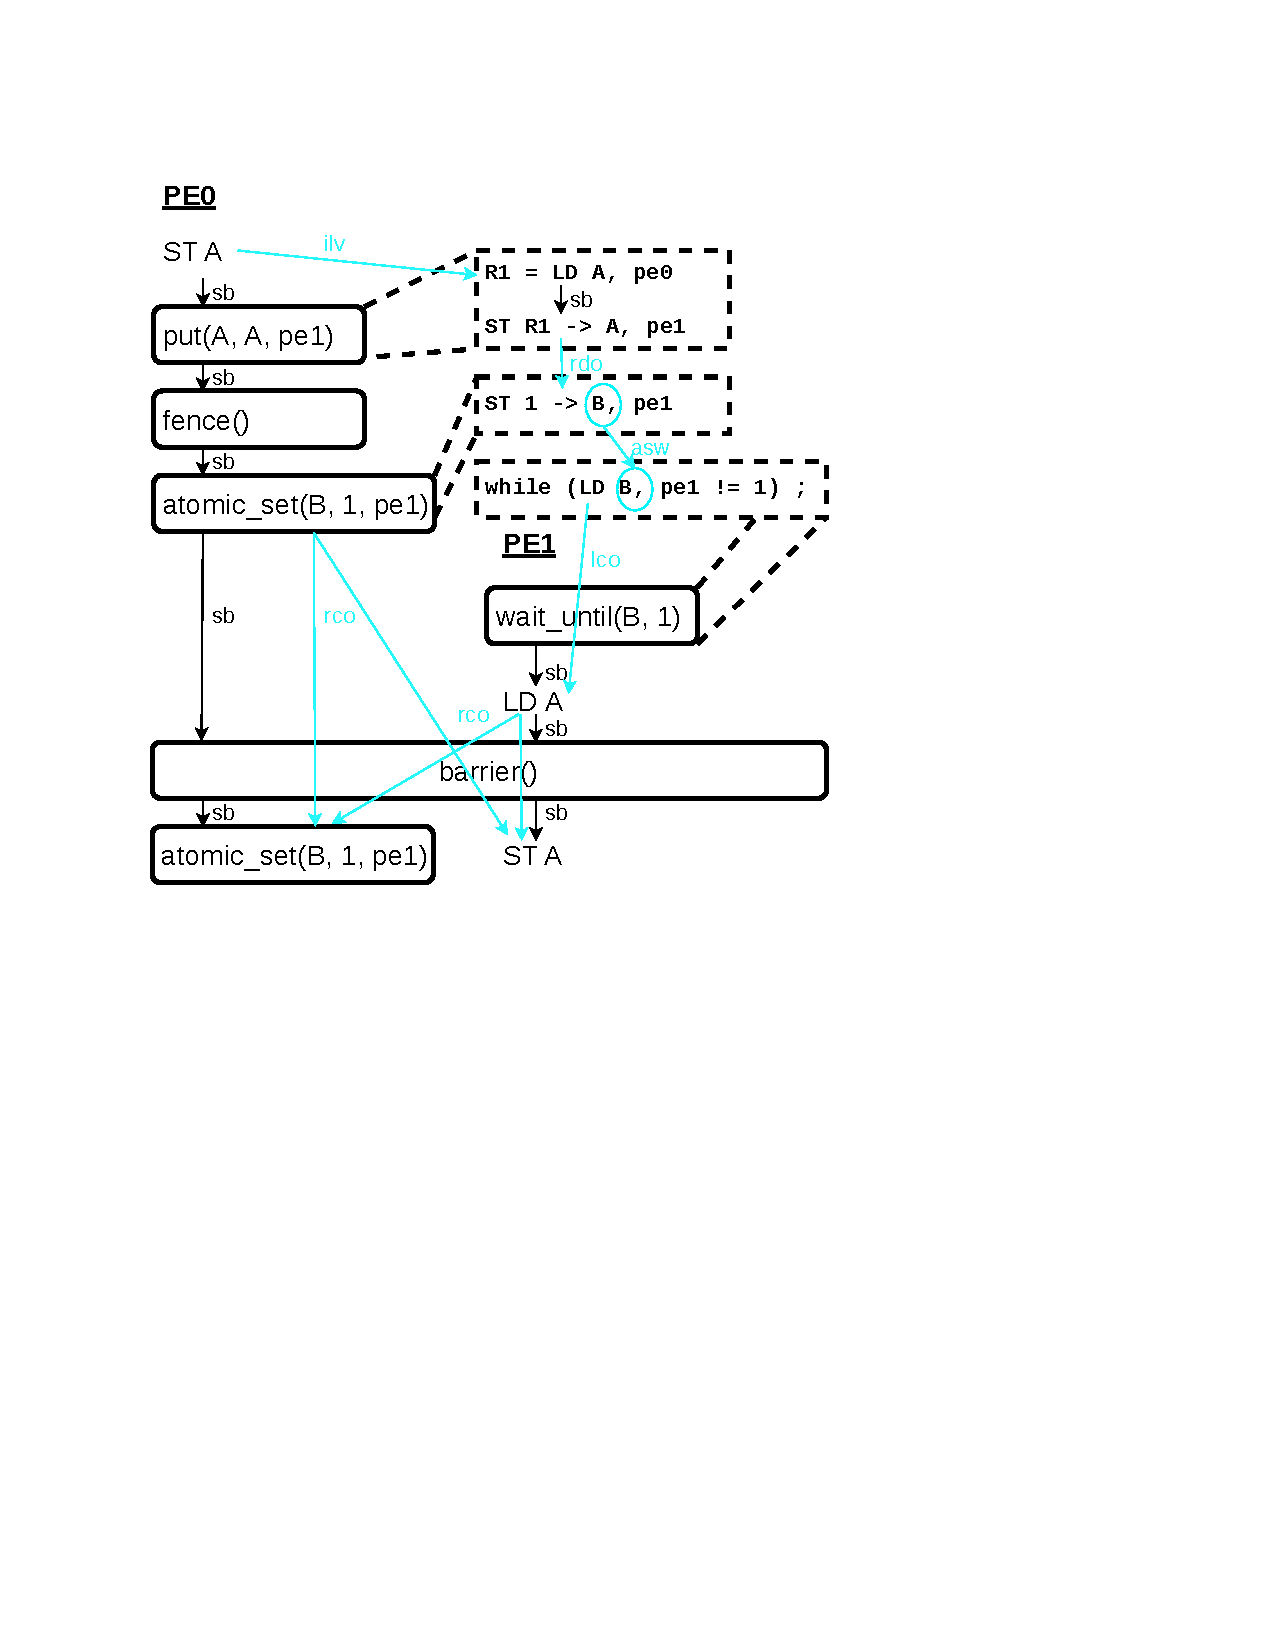
\includegraphics[width=0.75\textwidth]{figures/api_relations}
\centering
\caption{Example \openshmem code execution depicting observable accesses, example API-level relations, and a fused barrier collective operation event.}
\label{fig:api_execution}
\end{figure}

Figure~\ref{fig:api_execution} illustrates how the above concepts are applied in an example \openshmem code execution. \openshmem operations are denoted by rounded boxes, and their observable accesses are shown in dotted square boxes. 
Matched barrier calls from each \ac{PE} are fused into a single operation event.
Operations are ordered within the calling thread by \relSB{}, but their observable accesses are constrained only by the added API relations, described below (in addition to \relSB{} orderings within the operation): 
\begin{itemize}
\item \relILV{} orders the store of $a$ in PE0 (and all prior \relHB{}-ordered accesses) with the load of $a$ from the \PUT{} operation.
\item \relLCO{} orders the load of $a$ in PE1 (and all subsequent hb-ordered accesses) with the load of $b$ from the (blocking) \FUNC{wait\_until} operation.
\item \relRDO{} orders the bulk store of $a$ from the \PUT{} operation in PE0 with the store of $b$ from the fence-separated \FUNC{atomic\_set} operation.
\item \relRCO{} orders all \relHB{} ordered accesses and the accesses of \relHB{} ordered \openshmem operations before and after the fused barrier event spanning PE0 and PE1.
\item \relASW{} orders the store of $b$ from the \FUNC{atomic\_set} operation in PE0 with the consuming (\relRF{} related) load of $b$ from the \FUNC{wait\_until} operation in PE1.
\end{itemize}
Note that~\ref{fig:api_execution} depicts only a representative sample of API relations, since an exhaustive depiction would be cluttered.

\subsubsection{Updating the PL-Level Model to an API-Level Model}\label{subsubsec:api_integrate}

We leverage the newly defined observable accesses and ordering relations to define the API-level  memory model, which is based on the C11 model summarized in Section~\ref{subsubsec:api_pl_baseline}. 
We first define a new relation, \relAHB{} (\REL{api\_hb}), to be the transitive closure of the C11 \relHB{} and all API-level ordering relations introduced in Section~\ref{subsubsec:api_relations}:

\begin{itemize}
    \item $api\_hb := (hb \cup ilv \cup lco \cup rdo \cup rco \cup asw)^+$
\end{itemize}

In addition, an \relADR{} is defined to relate any two accesses $A$ and $B$ where all of the following are true:
\begin{itemize}
    \item $A$ and $B$ access the same memory location on the same \ac{PE}.
    \item At least one access is a modifying access (write or read-modify-write).
    \item Both $A$ and $B$ are normal accesses and at least one of them is not atomic, or both $A$ and $B$ are observable memory accesses issued by \openshmem operations and at least one of them is issued by a non-synchronizing \openshmem operation (defined in Section~\ref{subsubsec:api_relations}), or one of the accesses is a normal memory access and the other is an observable memory access issued by an \openshmem operation.
    \item $A$ and $B$ are not related by \relAHB{}.
\end{itemize}

The following axioms are similarly updated to use \relAHB{} rather than \relHB{}, and to extend RMW atomicity to \openshmem \ac{AMO}s:
\begin{itemize}
    \item $acyclic(api\_hb)$: \relAHB{} cannot have any cycles.
    \item $irreflexive(rf;api\_hb)$: \relAHB{} must be consistent with the \relRF{} relation.
    \item $irreflexive((rf^{-1})^{?};mo;rf^?;api\_hb)$: \relAHB{} must be consistent with \relMO{} between writes, and it must also be consistent with the order of reads that read from writes in \relMO{} (often called coherence requirement).
    \item $irreflexive(rf \cup (mo;mo;rf^{-1}) \cup (mo;rf))$: The read of an atomic read-modify-write access must always read the last value (in \relMO{}) written before the write of the read-modify-write access (often called RMW atomicity).
    \item $irreflexive(rf;sb^{amo\_op} \cup (mo;mo;(sb^{amo\_op})^{-1};rf^{-1}) \cup (mo;rf))$: The observable read of an \openshmem \ac{AMO} must always read the last value (in \relMO{}) written before the observable write of the \ac{AMO} (this is the \ac{AMO} analog of the PL-level RMW atomicity axiom). In this axiom, $sb^{amo\_op}$ is defined as the $sb$ relation between the observable read and write accesses issued by an \ac{AMO}.
    \item $irreflexive(rf \cup (mo;mo;rf^{-1}) \cup (mo;rf))$: The read of an atomic read-modify-write access must always read the last value (in \relMO{}) written before the write of the read-modify-write access.
\end{itemize}

Finally, similar to the C11 memory model, if an \relADR{} exists in a candidate execution that satisfies the above axioms, then the behavior is undefined. If an \relADR{} does not exist, then the behavior must conform to one of the axiom-satisfying candidate executions.

\subsubsection{Compatibility with a Scoped Memory Model}\label{subsubsec:api_scoped}

Memory models for accelerators like GPUs often extend CPU-oriented memory models like C11 with the notion of synchronization scopes. Scopes are necessary to enable efficient synchronization in a system with software-managed cache coherence. A scope is a property assigned to each atomic access that corresponds to a grouping of threads in a program execution. The threads in a grouping may share a cache in the cache hierarchy, such that communication between those threads can occur more efficiently at that cache level.
When synchronizing between two threads, the synchronizing accesses must use a scope that contains both synchronizing threads; if they do not, this represents a heterogeneous race in the scoped memory model, and program behavior is undefined.

Properly scoped synchronization is critical for GPU applications, but it is not necessary to expose it at the level of the \openshmem API. Scopes are important for communication between threads that share a cache level, but the threads participating in inter-PE communication governed by \openshmem generally do not share a cache.
Of course, implementing \openshmem operations may require synchronization and communication between threads in a \ac{PE} that can benefit from scopes, e.g., when offloading a non-blocking operation to a helper thread. However, this synchronization should be entirely performed within the \openshmem implementation transparently to the user of the \openshmem API. In this way, \openshmem users and implementers may freely and independently optimize their own code without agreeing on the relative locations of \openshmem helper threads.
This policy has the added benefit of retaining a single simple and portable API-level interface for \openshmem that may be applied on top of memory models that may or may not use scoped synchronization.
